\documentclass[12pt]{article}

\usepackage{amsmath, amssymb, amsthm}
\usepackage{algorithm, algpseudocode}
\usepackage{hyperref}
\usepackage{geometry}
\usepackage{graphicx}
\usepackage{tikz}
\usetikzlibrary{positioning, arrows.meta, shapes.geometric, calc}

\geometry{margin=1in}

\newtheorem{claim}{Claim}

\title{Method statement}
\author{Ilay Menahem}

\begin{document}

\maketitle

\section*{Introduction}

A Gr\"obner basis is the standard tool for analyzing a system of polynomial equations $p_1 = \cdots = p_m = 0$, but computing one can be infeasible for large systems.
In this document we therefore look for a weaker object: a Gr\"obner basis for a structured subvariety of $V(p_1, \ldots, p_m)$. Such a subvariety is obtained by adding optional structure hints, such as equations of the form $x_i = 0$, and by choosing one irreducible factor from each preprocessed polynomial.

\section*{The outer branching algorithm}

\begin{algorithm}
\caption{Outer branching}
\label{alg:Outer branching}
\begin{algorithmic}[1]
    \Require A set of polynomials $P = \{p_1, \ldots, p_m\}$ set of structure hints $H$.

    \State Interreduce the polynomials

    \State Initialize $C \gets \emptyset$ an unsatisfiable cores set
    \State Initialize $C_H \gets \emptyset$ an unsatisfiable structure-hint cores set
    \State Initialize $S \gets \emptyset$ a solutions set

    \For{Each subset of the structure hints $F \subseteq H$}
        \If{$F$ contains an unsatisfiable structure-hint core from $C_H$}
            \State \textbf{continue}
        \EndIf

        \State $P_F \gets P \cup F$
        \State Interreduce the polynomials in $P_F$
        \State Factor the polynomials in $P_F$ into irreducible factors $C_1, \ldots, C_m$

        \For{Each minimal hitting set $HS$ of $C_1, \ldots, C_m$}
            \If{$HS \cup F$ contains an unsatisfiable core from $C$}
                \State \textbf{continue}
            \EndIf

            \State Check if the minimal hitting set $HS \cup F$ is satisfiable
            \If{$HS \cup F$ is satisfiable}
                \State Add the solution to $S$
            \Else
                \State Extract a minimal unsatisfiable core $U$ from $HS \cup F$
                \State $C \gets C \cup \{U\}$
            \EndIf
        \EndFor

        \If{No minimal hitting set was satisfiable}
            \State $U_H \gets \Call{ExtractUnsatisfiableHintCore}{P, F}$
            \State $C_H \gets C_H \cup \{U_H\}$
            \State \textbf{continue}
        \EndIf
    \EndFor

    \Return $S$, $C$, and $C_H$

\end{algorithmic}
\end{algorithm}

\begin{algorithm}
\caption{Extracting a minimal unsatisfiable structure-hint core}
\label{alg:extracting a minimal unsatisfiable structure-hint core}
\begin{algorithmic}[1]
    \Require A polynomial system $P$ and a set of structure hints $F$ such that $P \cup F$ is unsatisfiable.

    \State $U_H \gets F$
    \For{each hint $h \in F$}
        \If{$P \cup (U_H \setminus \{h\})$ is unsatisfiable}
            \State $U_H \gets U_H \setminus \{h\}$
        \EndIf
    \EndFor

    \Return $U_H$

\end{algorithmic}
\end{algorithm}

\begin{algorithm}
\caption{Extracting a minimal unsatisfiable core}
\label{alg:extracting a minimal unsatisfiable core}
\begin{algorithmic}[1]
    \Require A set of constraints $F$ that is unsatisfiable.

    \State Initialize $U = F$
    \For{each constraint $f \in F$}
        \State $U' \gets U \setminus \{f\}$
        \State Check whether $U'$ is unsatisfiable
        \If{$U'$ is unsatisfiable}
            \State $U \gets U'$
        \EndIf
    \EndFor

    \Return $U$

\end{algorithmic}
\end{algorithm}

The order of iteration over the minimal hitting sets and the structure hints should heuristically prioritize the easier to check sets first.

\begin{figure}[H]
\centering
\resizebox{\textwidth}{!}{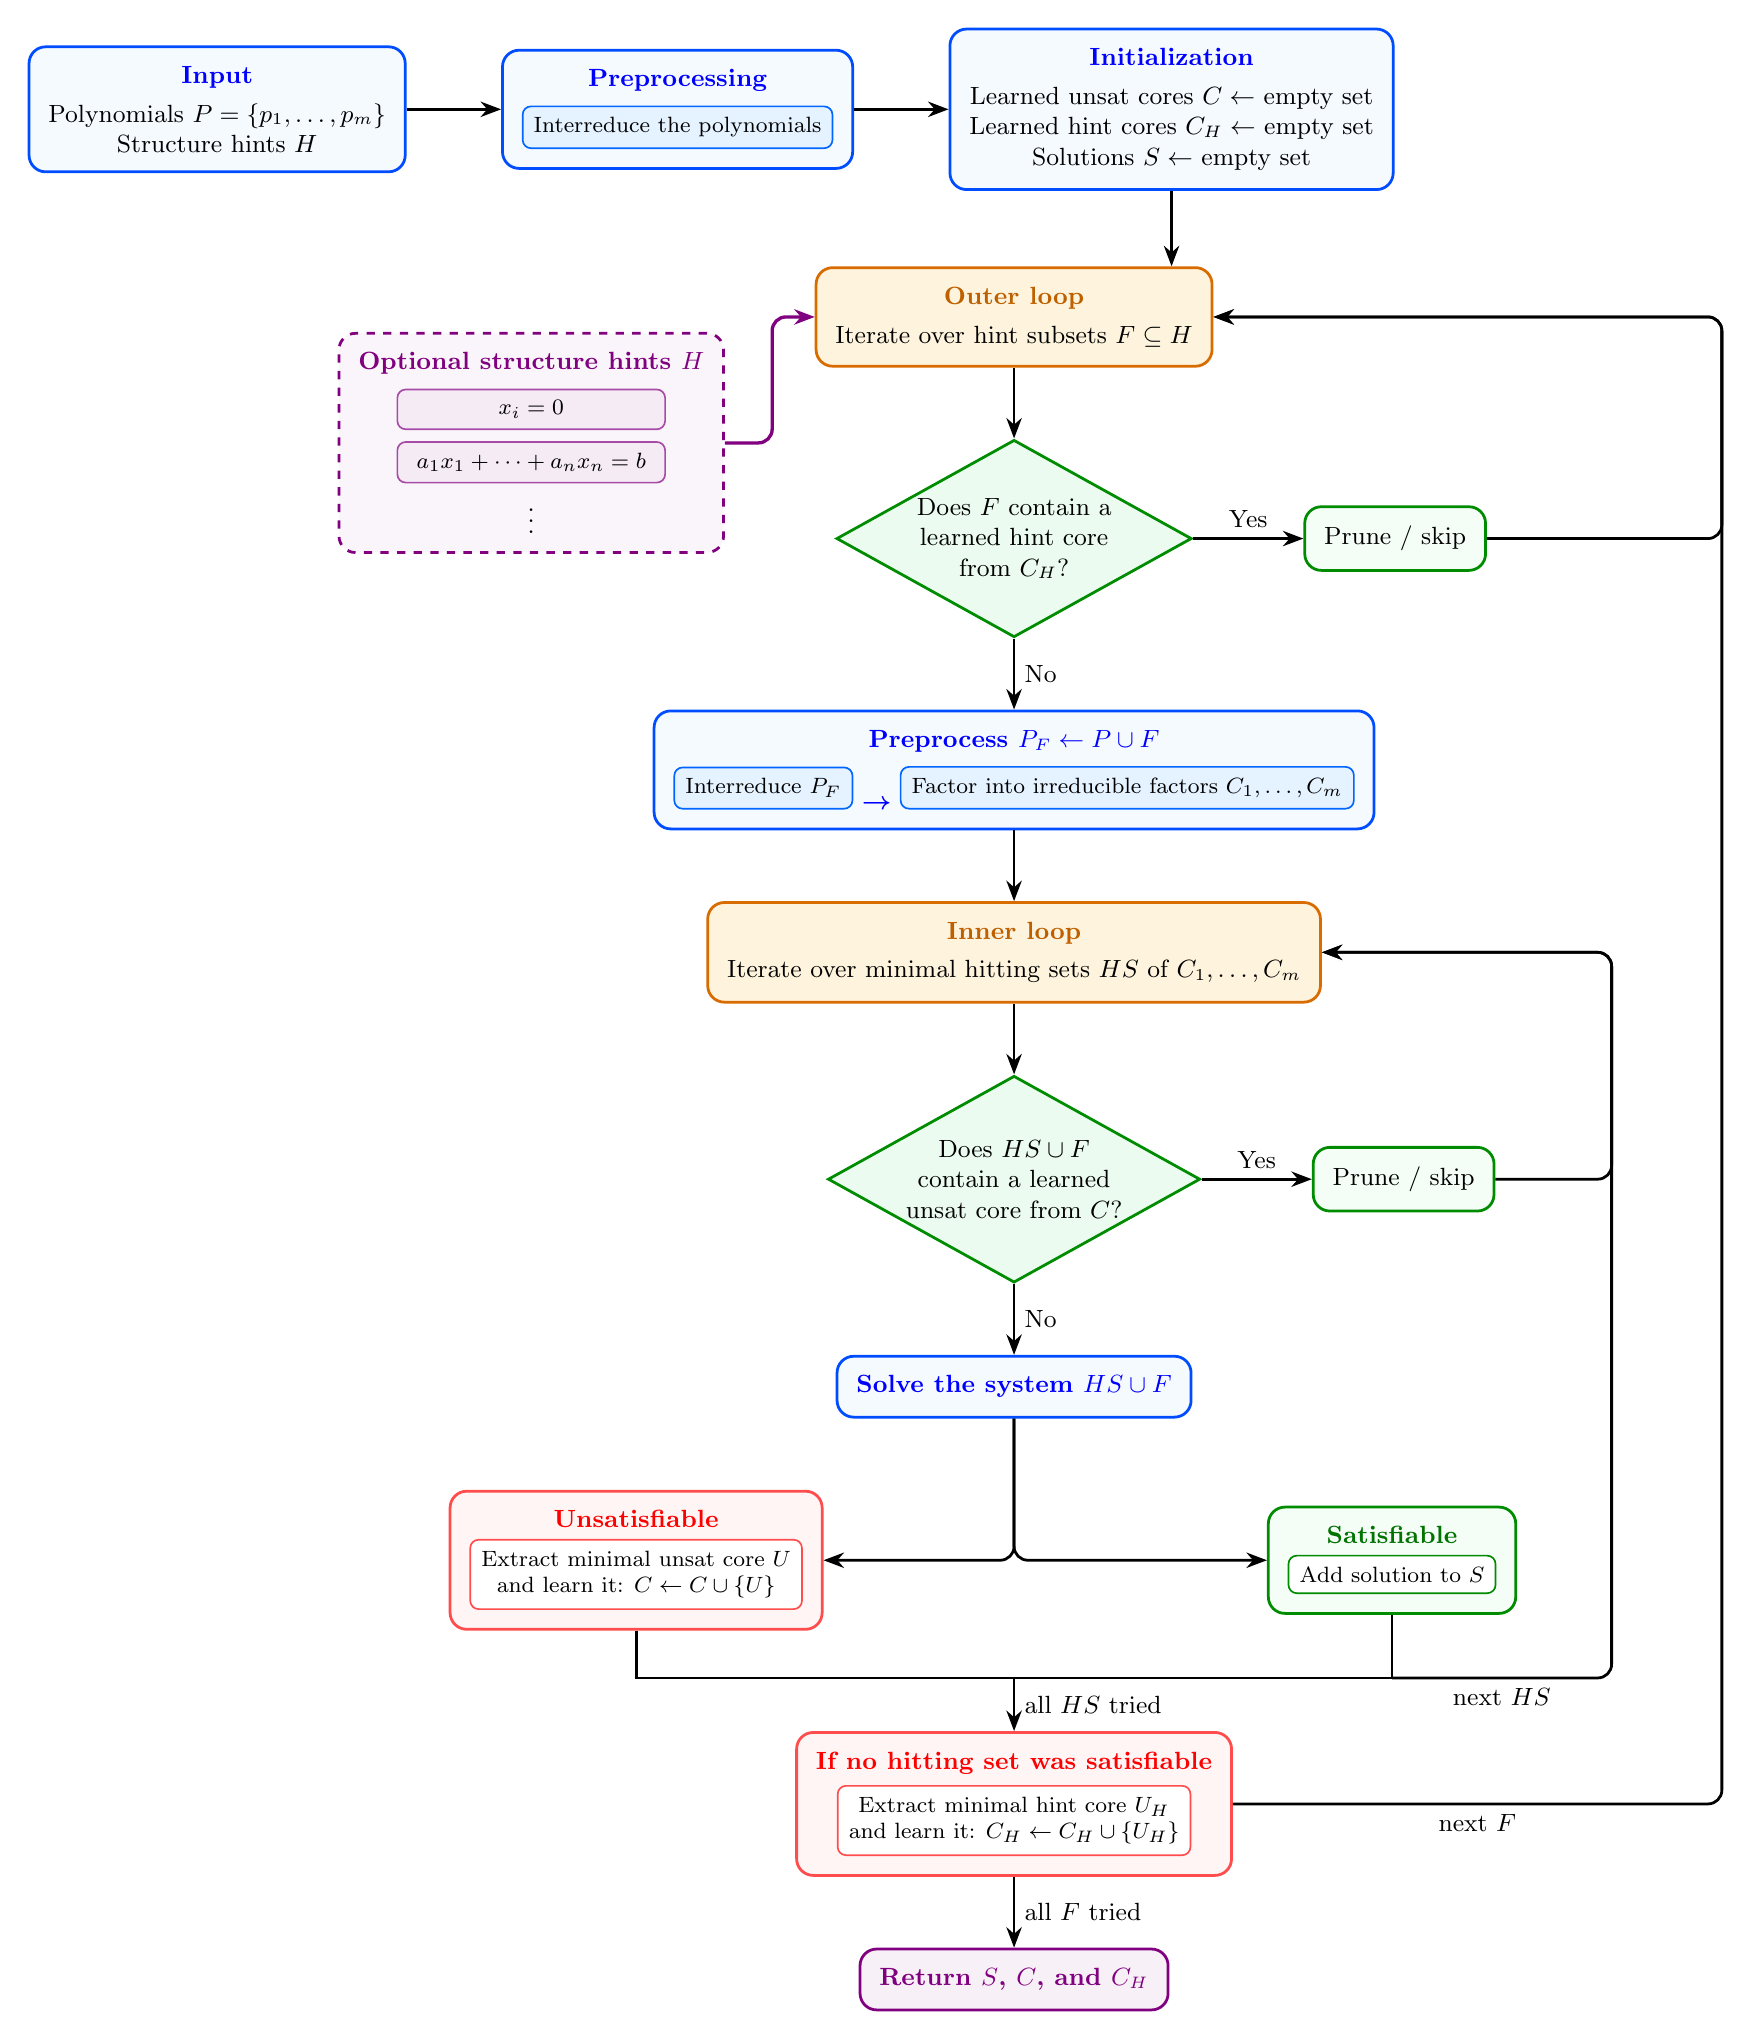
\begin{tikzpicture}[
    font=\small,
    every node/.style={align=center},
    blue box/.style={draw=blue!70!cyan, line width=1pt, rounded corners=6pt,
        fill=blue!50!cyan!4, inner sep=7pt},
    blue subbox/.style={draw=blue!60!cyan, line width=.6pt, rounded corners=3pt,
        fill=blue!50!cyan!10, inner sep=4pt, font=\footnotesize},
    loop box/.style={draw=orange!85!black, line width=1pt, rounded corners=6pt,
        fill=yellow!40!orange!12, inner sep=7pt},
    decision/.style={draw=green!55!black, line width=1pt, diamond, aspect=1.8,
        fill=green!60!teal!8, inner sep=1pt},
    green box/.style={draw=green!55!black, line width=1pt, rounded corners=6pt,
        fill=green!60!teal!4, inner sep=7pt},
    green subbox/.style={draw=green!55!black, line width=.6pt, rounded corners=3pt,
        fill=white, inner sep=4pt, font=\footnotesize},
    red box/.style={draw=red!70, line width=1pt, rounded corners=6pt,
        fill=red!4, inner sep=7pt},
    red subbox/.style={draw=red!70, line width=.6pt, rounded corners=3pt,
        fill=white, inner sep=4pt, font=\footnotesize},
    hint box/.style={draw=violet, dashed, line width=1pt, rounded corners=6pt,
        fill=violet!4, inner sep=7pt},
    hint subbox/.style={draw=violet!70, solid, line width=.6pt, rounded corners=3pt,
        fill=violet!8, inner sep=4pt, font=\footnotesize},
    return box/.style={draw=violet, line width=1pt, rounded corners=6pt,
        fill=violet!6, inner sep=7pt},
    arr/.style={-{Stealth[length=2.6mm]}, line width=1pt},
]

% ---- top row: input -> preprocessing -> initialization ----
\node[blue box] (input) {%
    \textcolor{blue}{\bfseries Input}\\[3pt]
    Polynomials $P = \{p_1,\ldots,p_m\}$\\
    Structure hints $H$};

\node[blue box, right=12mm of input] (prep) {%
    \textcolor{blue}{\bfseries Preprocessing}\\[4pt]
    \tikz{\node[blue subbox] {Interreduce the polynomials};}};

\node[blue box, right=12mm of prep] (init) {%
    \textcolor{blue}{\bfseries Initialization}\\[3pt]
    Learned unsat cores $C \leftarrow$ empty set\\
    Learned hint cores $C_H \leftarrow$ empty set\\
    Solutions $S \leftarrow$ empty set};

% ---- outer loop over hint subsets ----
\node[loop box] (outerloop) at ($(init.south)+(-20mm,-16mm)$) {%
    \textcolor{orange!75!black}{\bfseries Outer loop}\\[3pt]
    Iterate over hint subsets $F \subseteq H$};

% ---- optional structure hints ----
\node[hint box] (hints) at ($(outerloop.west)+(-36mm,-16mm)$) {%
    \textcolor{violet}{\bfseries Optional structure hints $H$}\\[4pt]
    \tikz{\node[hint subbox, minimum width=34mm] {$x_i = 0$};}\\[3pt]
    \tikz{\node[hint subbox, minimum width=34mm]
        {$a_1 x_1 + \cdots + a_n x_n = b$};}\\[2pt]
    $\vdots$};

% ---- hint-core decision + prune ----
\node[decision, below=9mm of outerloop] (hintcore) {%
    Does $F$ contain a\\ learned hint core\\ from $C_H$?};

\node[green box, right=14mm of hintcore] (pruneH) {Prune / skip};

% ---- per-subset preprocessing ----
\node[blue box, below=9mm of hintcore] (prepF) {%
    \textcolor{blue}{\bfseries Preprocess $P_F \gets P \cup F$}\\[4pt]
    \tikz{\node[blue subbox] {Interreduce $P_F$};}
    \textcolor{blue}{$\boldsymbol{\rightarrow}$}
    \tikz{\node[blue subbox] {Factor into irreducible factors $C_1,\ldots,C_m$};}};

% ---- inner loop over minimal hitting sets ----
\node[loop box, below=9mm of prepF] (innerloop) {%
    \textcolor{orange!75!black}{\bfseries Inner loop}\\[3pt]
    Iterate over minimal hitting sets $HS$ of $C_1,\ldots,C_m$};

% ---- unsat-core decision + prune ----
\node[decision, below=9mm of innerloop] (learned) {%
    Does $HS \cup F$\\ contain a learned\\ unsat core from $C$?};

\node[green box, right=14mm of learned] (prune) {Prune / skip};

% ---- solve ----
\node[blue box, below=9mm of learned] (solve) {%
    \textcolor{blue}{\bfseries Solve the system $HS \cup F$}};

% ---- unsat / sat branches ----
\node[red box] (unsat) at ($(solve.south)+(-48mm,-18mm)$) {%
    \textcolor{red}{\bfseries Unsatisfiable}\\[3pt]
    \tikz{\node[red subbox] {Extract minimal unsat core $U$ \\ and learn it: $C \leftarrow C \cup \{U\}$};}};

\node[green box] (sat) at ($(solve.south)+(48mm,-18mm)$) {%
    \textcolor{green!45!black}{\bfseries Satisfiable}\\[3pt]
    \tikz{\node[green subbox] {Add solution to $S$};}};

% ---- bottom rail ----
\coordinate (raill) at ($(unsat.south)+(0,-6mm)$);
\coordinate (railr) at (raill -| sat.south);

% ---- hint-core learning after the inner loop ----
\node[red box] (hintlearn) at ($($(raill)!0.5!(railr)$)+(0,-16mm)$) {%
    \textcolor{red}{\bfseries If no hitting set was satisfiable}\\[3pt]
    \tikz{\node[red subbox] {Extract minimal hint core $U_H$ \\
        and learn it: $C_H \leftarrow C_H \cup \{U_H\}$};}};

% ---- return ----
\node[return box, below=9mm of hintlearn] (return)
    {\textcolor{violet}{\bfseries Return $S$, $C$, and $C_H$}};

% ---- arrows: top pipeline ----
\draw[arr] (input) -- (prep);
\draw[arr] (prep) -- (init);
\draw[arr] (init.south) -- (init.south |- outerloop.north);

% ---- structure hints into the outer loop ----
\draw[arr, violet, line width=1.2pt, rounded corners=5pt]
    (hints.east) -- ++(6mm,0) |- (outerloop.west);

% ---- outer loop body ----
\draw[arr] (outerloop.south) -- (hintcore.north);
\draw[arr] (hintcore.east) -- node[above] {Yes} (pruneH.west);
\draw[arr] (hintcore.south) -- node[right] {No} (prepF.north);
\draw[arr] (prepF.south) -- (innerloop.north);

% ---- inner loop body ----
\draw[arr] (innerloop.south) -- (learned.north);
\draw[arr] (learned.east) -- node[above] {Yes} (prune.west);
\draw[arr] (learned.south) -- node[right] {No} (solve.north);
\draw[arr, rounded corners=5pt] (solve.south) |- (unsat.east);
\draw[arr, rounded corners=5pt] (solve.south) |- (sat.west);

% ---- bottom rail into hint-core learning and return ----
\draw[line width=1pt] (unsat.south) -- (raill) -- (railr) -- (sat.south);
\draw[arr] (hintlearn.north |- raill) --
    node[right] {all $HS$ tried} (hintlearn.north);
\draw[arr] (hintlearn) -- node[right] {all $F$ tried} (return);

% ---- inner feedback: next hitting set ----
\coordinate (fbcol) at ($(sat.east)+(12mm,0)$);
\draw[arr, rounded corners=5pt]
    (prune.east) -- (prune.east -| fbcol) |- (innerloop.east);
\draw[arr, rounded corners=5pt]
    (railr) -- node[below] {next $HS$} (railr -| fbcol) |- (innerloop.east);

% ---- outer feedback: next hint subset ----
\coordinate (fbcol2) at ($(sat.east)+(26mm,0)$);
\draw[arr, rounded corners=5pt]
    (pruneH.east) -- (pruneH.east -| fbcol2) |- (outerloop.east);
\draw[arr, rounded corners=5pt]
    (hintlearn.east) -- node[below] {next $F$}
    (hintlearn.east -| fbcol2) |- (outerloop.east);

\end{tikzpicture}
}
\caption{The CDCL pipeline specialized to a system of polynomial equations.}
\label{fig:cdcl flowchart}
\end{figure}

\subsection*{Minimal hitting sets of the factors}
\textbf{Order of iteration over the minimal hitting sets}: the order is from the simplest to the most complex to check for satisfiability. As a heuristic for this cost we use the rule more factors $\Rightarrow$ more complex to check, and more hints $\Rightarrow$ easier to check.

\subsection*{Finding the unsatisfiable cores}
To check if a set of polynomials $F$ is satisfiable, we compute its reduced Gr\"obner basis $G$ with respect to a degrevlex order, using a signiture based algorithm such as F5, M4GB, or GVW.

\textbf{unsatisfiable core} is a subset $U \subseteq F$ of factors with no common zero. We detect this from the reduced Gr\"obner basis of $U$, which equals $\{1\}$ exactly when $1 \in \langle U \rangle$.

If we were to select an hitting set $F$ that is contained in a previously found satisfiable hitting set $F'$, then $V(F) \supseteq V(F') \neq \emptyset$ and $F$ is also satisfiable. This is the dual of the unsatisfiable core property, and can be used to prune the search space in a similar way.

\subsection*{Using structure hints}

In some problems such as in physics, we prefer solutions which have certain structure.
certain structures can be encoded as additional polynomial constraints, and can enable faster computation of the Gr\"obner basis.

Structure hints also admit an additional form of unsatisfiability pruning.  For a chosen hint set $F \subseteq H$, we first check whether $P \cup F$ has a solution before branching over factors.  If it does not, we remove hints one at a time while the remaining system stays unsatisfiable, obtaining a minimal subset $U_H \subseteq F$ such that $P \cup U_H$ has no solution.  Every hint set $F' \supseteq U_H$ is then unsatisfiable as well, so all such sets can be skipped.

\begin{itemize}
    \item Sparsity constrains can be encoded as the equation $x_i = 0$ for some variables $x_i$
    \item Affine constraints can be encoded as $a_1 x_1 + \cdots + a_n x_n = b$ for some constants $a_i, b$
\end{itemize}

\end{document}
